%
% winkeldreiteilung.tex
%
% (c) 2021 Prof Dr Andreas Müller, OST Ostschweizer Fachhochschule
%
\begin{frame}[t]
\setlength{\abovedisplayskip}{5pt}
\setlength{\belowdisplayskip}{5pt}
\frametitle{Winkeldreiteilung}
\vspace{-20pt}
\begin{columns}[t,onlytextwidth]
\begin{column}{0.43\textwidth}
\begin{center}
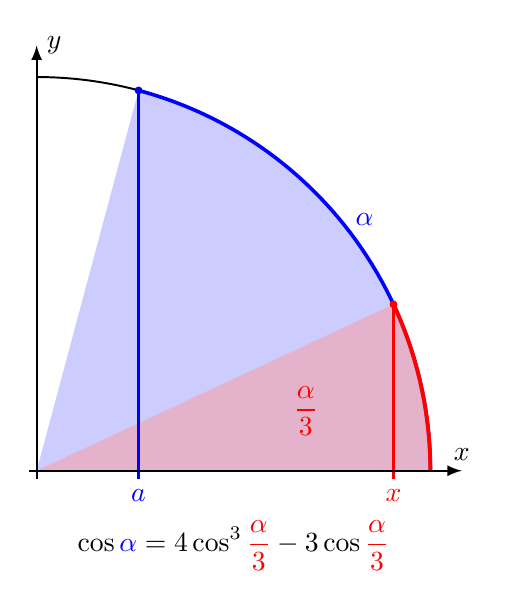
\begin{tikzpicture}[>=latex,thick]
\def\r{5}
\def\a{25}

\uncover<3->{
	\draw[line width=0.7pt] (\r,0) arc (0:90:\r);
}

\fill[color=blue!20] (0,0) -- (\r,0) arc(0:{3*\a}:\r) -- cycle;
\node[color=blue] at ({1.5*\a}:{1.05*\r}) {$\alpha$};

\draw[color=blue,line width=1.3pt] (\r,0) arc (0:{3*\a}:\r);

\uncover<2->{
	\fill[color=red!40,opacity=0.5] (0,0) -- (\r,0) arc(0:\a:\r) -- cycle;
	\draw[color=red,line width=1.4pt] (\r,0) arc (0:\a:\r);
	\node[color=red] at ({0.5*\a}:{0.7*\r})
		{$\displaystyle\frac{\alpha}{3}$};
}

\uncover<3->{
	\fill[color=blue] ({3*\a}:\r) circle[radius=0.05];
	\draw[color=blue] ({3*\a}:\r) -- ({\r*cos(3*\a)},-0.1);

	\fill[color=red] ({\a}:\r) circle[radius=0.05];
	\draw[color=red] ({\a}:\r) -- ({\r*cos(\a)},-0.1);

	\draw[->] (-0.1,0) -- ({\r+0.4},0) coordinate[label={$x$}];
	\draw[->] (0,-0.1) -- (0,{\r+0.4}) coordinate[label={right:$y$}];
}


\uncover<4->{
\node at ({0.5*\r},-0.5) [below] {$\displaystyle
\cos{\color{blue}\alpha}
=
4\cos^3{\color{red}\frac{\alpha}3} -3 \cos {\color{red}\frac{\alpha}3}
$};
}

\uncover<5->{
	\node[color=blue] at ({\r*cos(3*\a)},0) [below] {$a\mathstrut$};
	\node[color=red] at ({\r*cos(\a)},0) [below] {$x\mathstrut$};
}

\end{tikzpicture}
\end{center}
\end{column}
\begin{column}{0.53\textwidth}
\begin{block}{Aufgabe}
Teile einen Winkel in drei gleiche Teile
\end{block}
\vspace{-2pt}
\uncover<6->{%
\begin{block}{Algebraisierte Aufgabe}
Konstruiere $x$ aus $a$ derart, dass
\[
p(x)
=
x^3-\frac34 x -a = 0
\]
\uncover<7->{%
$a=0$:}
\uncover<8->{$p(x) = x(x^2-\frac{3}{4})\uncover<9->{\Rightarrow x = \frac{\sqrt{3}}2}$}
\end{block}}
\vspace{-2pt}
\uncover<10->{%
\begin{proof}[Unmöglichkeitsbeweis]
\begin{itemize}
\item<11->
$a\ne 0$ $\Rightarrow$  $p(x)$ irreduzibel
\item<12->
$p(x)$ definiert eine Körpererweiterung vom Grad $3$
\item<13->
Konstruierbar sind nur Körpererweiterungen vom Grad $2^l$
\qedhere
\end{itemize}
\end{proof}}
\end{column}
\end{columns}
\end{frame}
